
\documentclass{article}
\usepackage[utf8]{inputenc}
\usepackage{graphicx}
\usepackage{listings}
\usepackage{xcolor}
\usepackage{float}  % Add float package to control figure placement
\usepackage{amsmath}

\title{09c Building an Ultrasonic Sensor Alarm with a Keypad and Piezo Buzzer}
\author{Nicholas Bruzzese}
\date{\today}

\definecolor{dkgreen}{rgb}{0,0.6,0}
\definecolor{gray}{rgb}{0.5,0.5,0.5}
\definecolor{mauve}{rgb}{0.58,0,0.82}

\lstset{frame=tb,
	language=Python,
	aboveskip=3mm,
	belowskip=3mm,
	showstringspaces=false,
	columns=flexible,
	basicstyle={\small\ttfamily},
	numbers=none,
	numberstyle=\tiny\color{gray},
	keywordstyle=\color{blue},
	commentstyle=\color{dkgreen},
	stringstyle=\color{mauve},
	breaklines=true,
	breakatwhitespace=true,
	tabsize=3
}

\begin{document}
	
	\maketitle
	
	\section*{Introduction}
	In this lesson, you’ll learn how to build an alarm system using an ultrasonic sensor, a piezo buzzer, and a 4x4 keypad with a Raspberry Pi. The system monitors distance using the ultrasonic sensor and triggers an alarm when motion is detected. The alarm can only be deactivated by entering the correct PIN code on the keypad.
	
	\section*{Objectives}
	By the end of this lesson, you will:
	\begin{enumerate}
		\item Understand how to use an ultrasonic sensor to measure distance.
		\item Learn how to use a keypad for user input.
		\item Control a piezo buzzer to simulate an alarm.
		\item Combine components to create a functional alarm system.
	\end{enumerate}
	
	\section*{Hardware Requirements}
	\begin{itemize}
		\item Raspberry Pi (any model with GPIO pins).
		\item HC-SR04 Ultrasonic Sensor.
		\item 4x4 Keypad.
		\item Piezo buzzer.
		\item Jumper wires.
	\end{itemize}
	
	\section*{Hardware Setup}
	\subsection*{Component Connections}
	\begin{center}
		\begin{tabular}{|l|l|l|}
			\hline
			\textbf{Component}             & \textbf{Pin Name}   & \textbf{GPIO Pin}      \\
			\hline
			\textbf{Ultrasonic Sensor}     & \textbf{TRIG}       & GPIO 6                 \\
			& \textbf{ECHO}       & GPIO 5                 \\
			\textbf{Keypad}                & \textbf{Row 1 (L1)} & GPIO 5                 \\
			& \textbf{Row 2 (L2)} & GPIO 6                 \\
			& \textbf{Row 3 (L3)} & GPIO 13                \\
			& \textbf{Row 4 (L4)} & GPIO 19                \\
			& \textbf{Column 1 (C1)} & GPIO 12              \\
			& \textbf{Column 2 (C2)} & GPIO 16              \\
			& \textbf{Column 3 (C3)} & GPIO 20              \\
			& \textbf{Column 4 (C4)} & GPIO 21              \\
			\textbf{Piezo Buzzer}          & Positive            & GPIO 18                \\
			& Negative            & GND                    \\
			\hline
		\end{tabular}
	\end{center}
	
	\newpage
	\section*{Wiring Diagram}
	\begin{figure}[H]
		\centering
		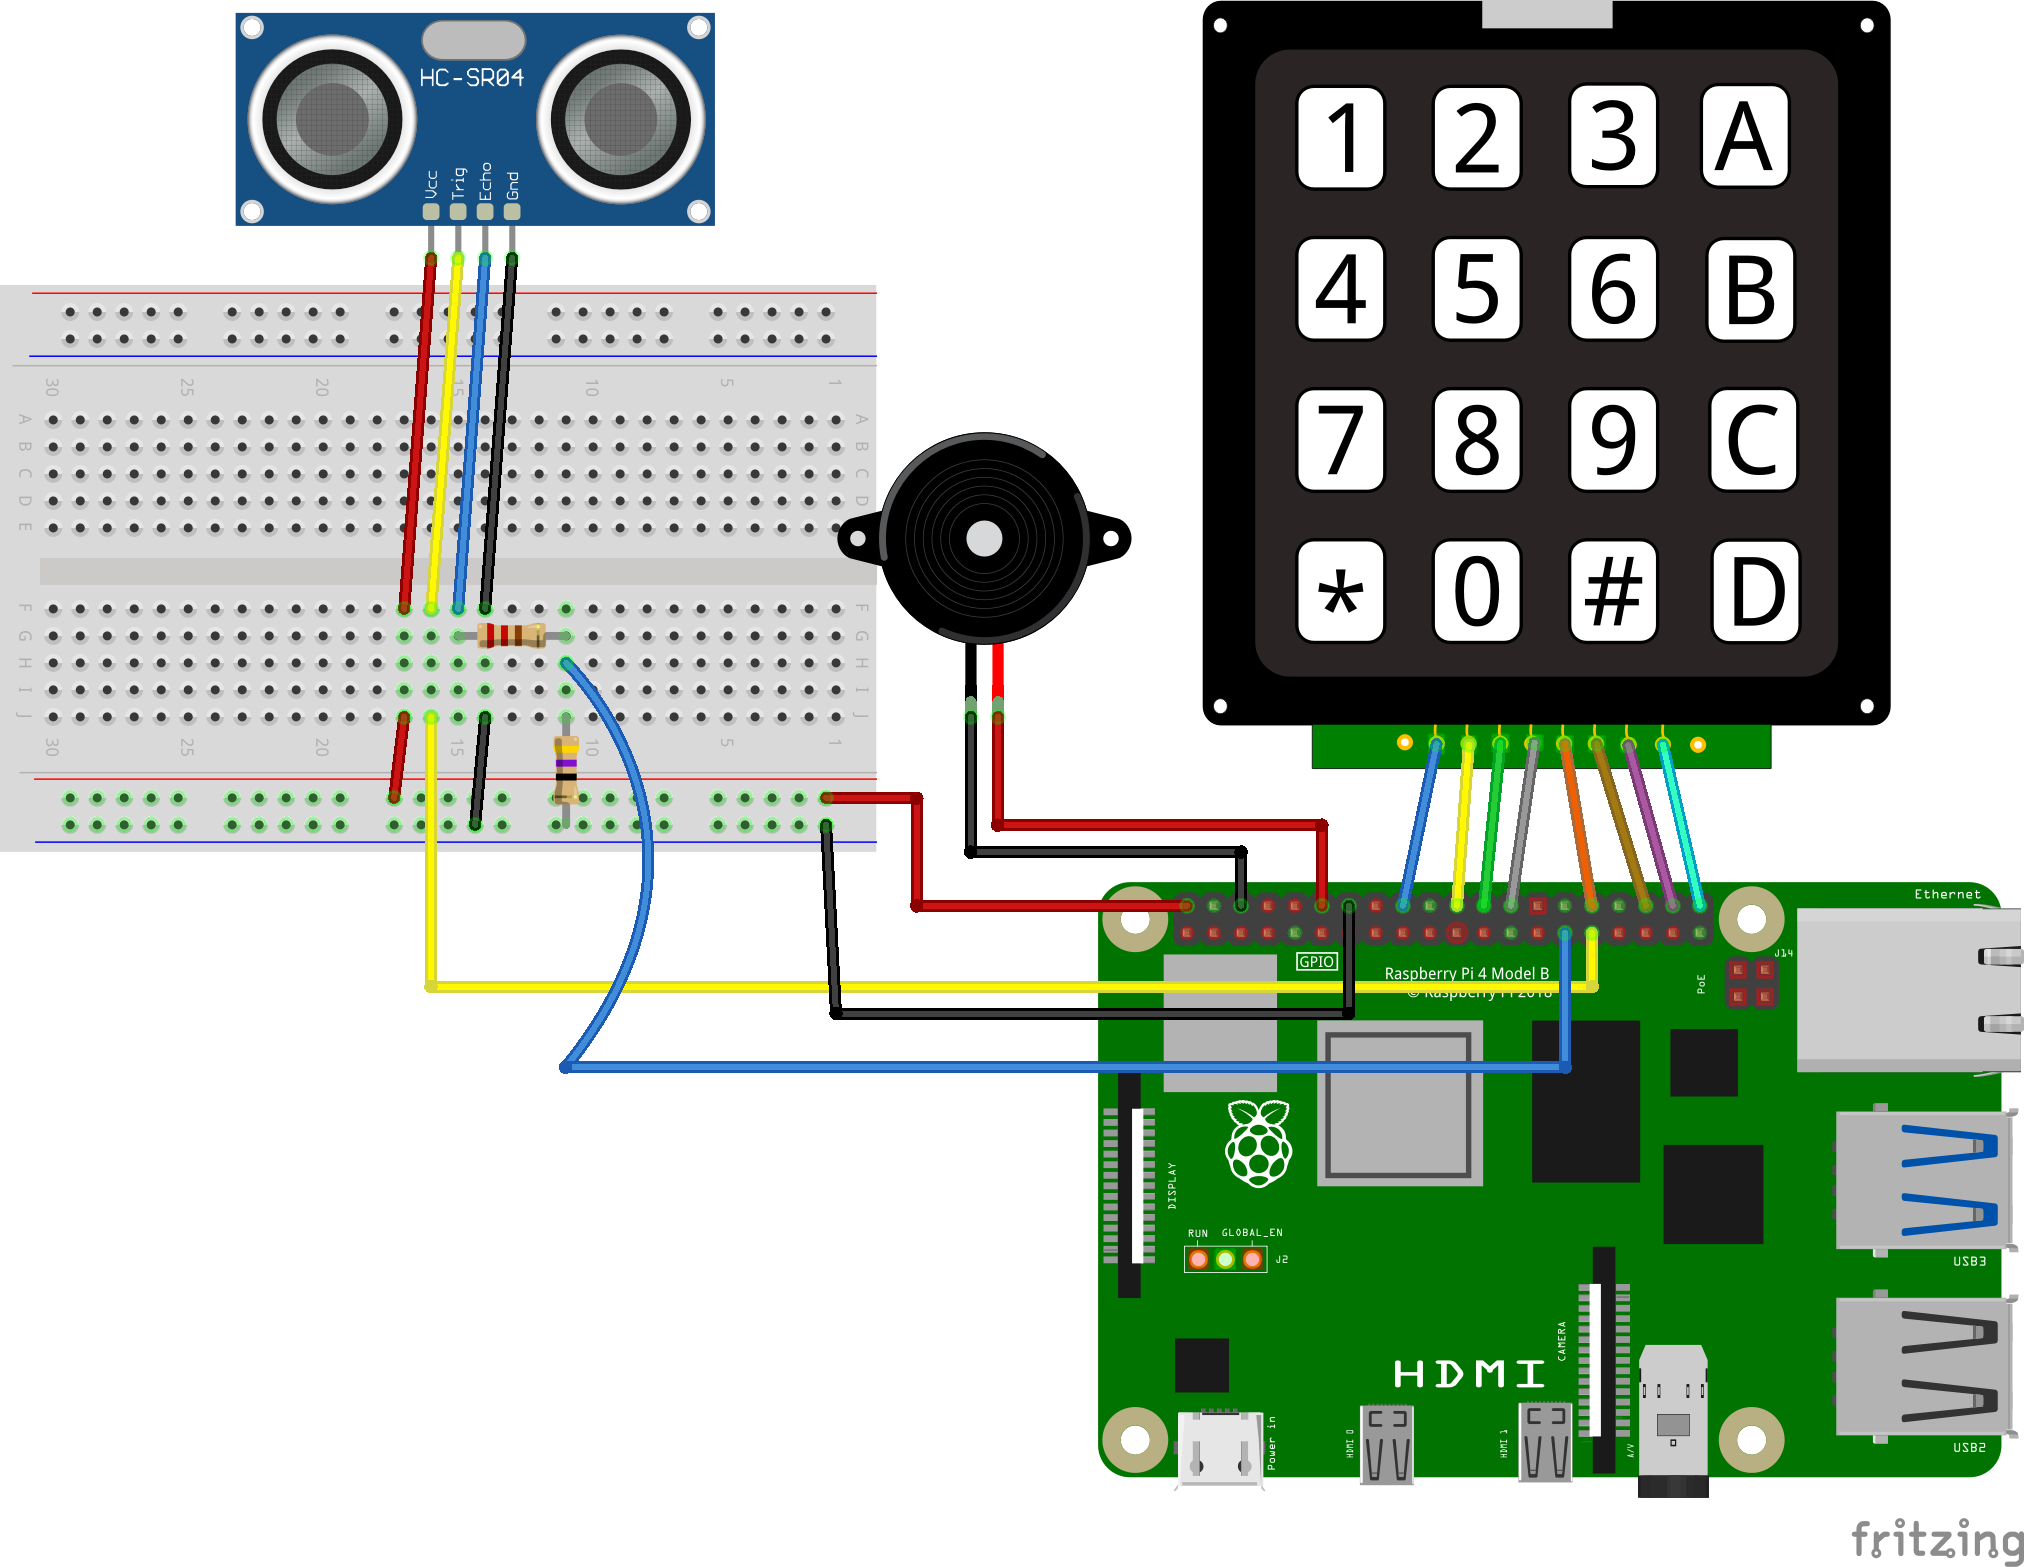
\includegraphics[width=1.2\textwidth]{09c-keypad-piezo-buzzer-us.png} % Adjust width to 80% of text width
		\caption{Wiring Diagram}
	\end{figure}
	
	\newpage
	\section*{Code Walkthrough}
	The Python code combines the functionality of the ultrasonic sensor, keypad, and piezo buzzer to create the alarm system.
	
	\subsection*{1. GPIO Initialization}
	The code initializes the GPIO pins for the ultrasonic sensor, keypad, and buzzer. The ultrasonic sensor measures distance, the keypad accepts user input, and the buzzer serves as the alarm.
	
	\begin{lstlisting}
		# Initialize GPIO
		GPIO.setwarnings(False)
		GPIO.setmode(GPIO.BCM)
		
		# Setup ultrasonic sensor GPIO pins
		GPIO.setup(TRIG, GPIO.OUT)
		GPIO.setup(ECHO, GPIO.IN)
		
		# Setup keypad GPIO pins
		GPIO.setup([L1, L2, L3, L4], GPIO.OUT)
		GPIO.setup([C1, C2, C3, C4], GPIO.IN, pull_up_down=GPIO.PUD_DOWN)
		
		# Setup buzzer GPIO pin
		GPIO.setup(BUZZER, GPIO.OUT)
	\end{lstlisting}
	
	\subsection*{2. Measuring Distance}
	The \texttt{measure\_distance()} function sends a pulse from the TRIG pin and calculates the time it takes for the echo to return to the ECHO pin. The function then converts this time into a distance in centimeters.
	
	\begin{lstlisting}
		def measure_distance():
		"""Measure distance using the ultrasonic sensor."""
		GPIO.output(TRIG, True)
		time.sleep(0.00001)
		GPIO.output(TRIG, False)
		
		while GPIO.input(ECHO) == 0:
		pulse_start = time.time()
		
		while GPIO.input(ECHO) == 1:
		pulse_end = time.time()
		
		pulse_duration = pulse_end - pulse_start
		distance = pulse_duration * 17150  # Speed of sound: 34300 cm/s
		return round(distance, 2)
	\end{lstlisting}
	
	\subsection*{3. Activating and Deactivating the Buzzer}
	The \texttt{buzz()} function controls the buzzer state. It turns the buzzer on or off based on the \texttt{state} parameter.
	
	\begin{lstlisting}
		def buzz(state):
		"""Turn the buzzer on or off."""
		GPIO.output(BUZZER, state)
	\end{lstlisting}
	
	\subsection*{4. Keypad Input}
	The \texttt{read\_line()} function scans the keypad for user input. If a key is pressed, it calls the \texttt{process\_key()} function to handle the input.
	
	\begin{lstlisting}
		def read_line(line, characters):
		"""Read input from the keypad."""
		global input_code, alarm_active
		
		GPIO.output(line, GPIO.HIGH)
		if GPIO.input(C1) == 1:
		process_key(characters[0])
		if GPIO.input(C2) == 1:
		process_key(characters[1])
		if GPIO.input(C3) == 1:
		process_key(characters[2])
		if GPIO.input(C4) == 1:
		process_key(characters[3])
		GPIO.output(line, GPIO.LOW)
	\end{lstlisting}
	
	\subsection*{5. Processing Keypad Input}
	The \texttt{process\_key()} function checks the user input against the predefined PIN code. If the input matches, it deactivates the alarm and stops the buzzer.
	
	\begin{lstlisting}
		def process_key(key):
		"""Handle key press events."""
		global input_code, alarm_active
		
		if alarm_active:
		print(f"Key pressed: {key}")
		input_code += key
		
		if len(input_code) >= len(PIN_CODE):
		if input_code == PIN_CODE:
		print("Correct PIN entered. Alarm deactivated.")
		buzz(False)
		alarm_active = False
		else:
		print("Incorrect PIN. Try again.")
		input_code = ""
	\end{lstlisting}
	
	\subsection*{6. Main Loop}
	The main loop monitors the ultrasonic sensor for motion and activates the alarm when an object is detected within the threshold distance. It also continuously checks the keypad for PIN entry.
	
	\begin{lstlisting}
		try:
		print("System initialized. Monitoring for motion...")
		
		while True:
		distance = measure_distance()
		print(f"Distance: {distance} cm")
		
		if distance < DISTANCE_THRESHOLD and not alarm_active:
		print("Motion detected! Alarm triggered!")
		buzz(True)
		alarm_active = True
		
		if alarm_active:
		read_line(L1, ["1", "2", "3", "A"])
		read_line(L2, ["4", "5", "6", "B"])
		read_line(L3, ["7", "8", "9", "C"])
		read_line(L4, ["*", "0", "#", "D"])
		
		time.sleep(0.1)
		
		except KeyboardInterrupt:
		print("\nApplication stopped!")
		
		finally:
		GPIO.cleanup()
	\end{lstlisting}
	
	\section*{Testing}
	\begin{enumerate}
		\item \textbf{Trigger the Alarm}: Place an object within 30 cm of the ultrasonic sensor. The buzzer should activate, indicating the alarm is triggered.
		\item \textbf{Deactivate the Alarm}: Enter the PIN (\texttt{1234}) on the keypad. The buzzer should stop, and the system should return to monitoring mode.
	\end{enumerate}
	
	\section*{Experiment Ideas}
	\begin{itemize}
		\item \textbf{Adjust Distance Threshold}: Change the \texttt{DISTANCE\_THRESHOLD} to make the system more or less sensitive.
		\item \textbf{Add LED Indicators}: Use LEDs to indicate system status (e.g., green for monitoring, red for alarm).
		\item \textbf{Custom Alarm Sound}: Modify the buzzer to play different tones or patterns when triggered.
		\item \textbf{Data Logging}: Record motion detection events to a file or database.
	\end{itemize}
	
	With this setup, you've created a versatile and functional alarm system that combines multiple Raspberry Pi components. Let me know if you have questions or want to expand this project!
	
\end{document}
